\section{Evaluation}
\label{sec:evaluation}

We evaluate \tool{} on real protocol implementations and answer five research
questions:
\begin{itemize}[leftmargin=*]
  \item \textbf{RQ1: Rule extraction.} Can field-centric extraction produce a
  stable rule set for each protocol standard?
  \item \textbf{RQ2: Rule-to-code alignment.} How accurately does \tool{} map a
  standard rule to implementation variables and contexts?
  \item \textbf{RQ3: Bug finding.} How many conformance-deviation reports does
  \tool{} submit, and how many are confirmed, fixed, rejected, pending, or
  assigned CVEs?
  \item \textbf{RQ4: Cost.} What is the LLM cost of generating submitted
  reports under GPT-5.4 pricing?
  \item \textbf{RQ5: Ablation.} Which system components are responsible for the
  observed performance?
\end{itemize}

\subsection{Subjects and Baselines}

Table~\ref{tab:protocol-implementations} lists the evaluated subjects. A key evaluation rule is
that \emph{all implementations of the same protocol version share the same rule
set}. For example, the TLS 1.3 implementations are checked against the same 312
rules extracted from RFC 8446, and the two QUIC implementations are checked
against the same 286 rules extracted from RFC 9000. This avoids accidentally
crediting \tool{} with more or fewer opportunities simply because an
implementation is easier to analyze.
The TLS/DTLS subjects include OpenSSL~\cite{openssl},
wolfSSL~\cite{wolfssl}, Mbed TLS~\cite{mbedtls}, openHiTLS, and
BoringSSL~\cite{boringssl}. The QUIC subjects are quiche~\cite{quiche} and
ngtcp2~\cite{ngtcp2}; the MQTT subjects are Mosquitto~\cite{mosquitto} and
wolfMQTT~\cite{wolfmqtt}; and the CoAP subject is libcoap~\cite{libcoap}.

\begin{table}[t]
\centering
\caption{Protocol implementations used for evaluation.}
\label{tab:protocol-implementations}
\resizebox{\columnwidth}{!}{
\begin{tabular}{lcccl}
\toprule
\textbf{Subject} & \textbf{Version} & \textbf{LoC} & \textbf{Protocol} & \textbf{Specification} \\
\midrule
OpenSSL   & 11b7b6e & 1456.3K & TLS 1.3    & RFC 8446 \\
wolfSSL   & 1d363f3 & 520.4K  & TLS 1.3    & RFC 8446 \\
Mbed TLS  & 0fe989b & 310.8K  & TLS 1.3    & RFC 8446 \\
openHiTLS & 3d295814 & 480.2K & TLS 1.3    & RFC 8446 \\
Mosquitto & 99fa50f & 180.6K  & MQTT 5.0   & MQTT 5.0 \\
Mosquitto & 99fa50f & 180.6K  & MQTT 3.1.1 & MQTT 3.1.1 \\
wolfMQTT  & 88d37ed & 41.5K   & MQTT 3.1.1 & MQTT 3.1.1 \\
quiche    & 851533c & 92.3K   & QUIC       & RFC 9000 \\
ngtcp2    & 4af1c77 & 130.1K  & QUIC       & RFC 9000 \\
libcoap   & 7bc9a41 & 115.0K  & CoAP       & RFC 7252 \\
BoringSSL & 7f4d9a2 & 760.4K  & DTLS 1.3   & RFC 9147 \\
\bottomrule
\end{tabular}
}
\end{table}

We compare \tool{} against four baselines under the same subject versions,
rule budgets, model family, temperature setting, and maximum reasoning rounds.
\textbf{Direct Agent} receives the relevant standard section plus the top
keyword-retrieved code snippets and is asked to produce conformance reports
without field-space construction. \textbf{LLM+RAG} uses the same prompt schema
but retrieves code by embedding similarity over function-level chunks.
\textbf{Static-only} keeps \tool{}'s rule and code indexes but replaces LLM
semantic filtering and reasoning with deterministic alias, token-overlap, and
error-path heuristics. \textbf{w/o Test Agent} runs the full pipeline but does
not attempt executable validation. Each baseline uses the same top-8 file,
top-20 variable, top-12 snippet, and three-round evidence budget unless that
component is absent by design; prompt templates and raw outputs are included in
the artifact.

\subsection{Metrics and Ground Truth}

For rule extraction, we report the number of extracted fields and rules per
protocol. For alignment, we use Var@1, Var@3, Ctx@1, Ctx@3, MRR, and average
token consumption. For bug finding, we distinguish four states. A
\emph{submitted report} is an issue we sent to a maintainer with a standard
span, normalized rule, code evidence, and reproduction material when available.
A \emph{confirmed fixed} report is a submitted report that the maintainer fixed
or explicitly confirmed as fixed. A \emph{false positive} is a submitted report
rejected by maintainer feedback, independent expert adjudication, or a
reproducible counter-test. A \emph{pending} report has not yet received enough
external signal for final adjudication. A CVE is counted only for previously
unknown vulnerabilities assigned CVE identifiers after disclosure.

Our precision denominator is the adjudicated subset, not all submitted reports:
$\mathrm{P}_{adj}=\mathrm{Confirmed}/(\mathrm{Confirmed}+\mathrm{FP})$.
Pending reports are excluded from this precision because treating them as true
or false would make the metric depend on maintainer response latency. We do not
claim whole-corpus recall for bug finding: exhaustively proving the absence of
all missed protocol deviations across all rules and implementations is outside
the evidence available in this study. For ablations, recall is therefore
reported only against the 126 confirmed-fixed reports as a fixed discovery set,
and is labeled \emph{coverage} rather than global recall. The full system
itself defines this reference set, so its coverage is not used as evidence of
complete discovery.

Alignment labels were built independently from bug-finding outcomes. We sampled
312 rule-implementation pairs stratified by protocol and subject. Two authors
with protocol and systems experience independently marked the correct
implementation variable and the minimal context that establishes the rule's
behavior. Disagreements were resolved by joint review of the standard span,
callers, validation helpers, and tests. A context is correct if it contains the
field representation and the relevant check, propagation, or error path; when
evidence is split across functions, any top-$k$ bundle that includes the
decisive callee and caller is counted as correct.

Bug reports are adjudicated at the granularity of a unique
rule-implementation violation after duplicate reports are merged. Each report
is first reviewed by two authors against the normalized rule, standard span,
code path, and validation logs. Reports with executable counterexamples are
marked test-confirmed before disclosure. Reports without executable
counterexamples are submitted only when the code evidence covers the parser,
validator, caller, and configuration path relevant to the rule. Maintainer
responses override author labels when they explain an implementation-specific
exception, reject the report with evidence, or land a patch. The review was not
blind because the evidence bundle necessarily identifies the rule and code
location; to reduce circularity, pending reports are excluded from precision
and no global recall is claimed.

\subsection{RQ1: Field-Centric Rule Extraction}

Table~\ref{tab:field-rule-statistics} follows the structure of the original
experiment table. \tool{} extracts the largest and most stable rule set because
variables are searched before rule extraction. The same protocol-level rules
are then reused for all implementations of that protocol version.

\begin{table}[t]
\centering
\caption{Statistics of extracted field-centric rules.}
\label{tab:field-rule-statistics}
\small
\setlength{\tabcolsep}{5pt}
\begin{tabular}{lrr|rr|rr}
\toprule
\textbf{Protocol}
& \multicolumn{2}{c|}{\textbf{0-shot}}
& \multicolumn{2}{c|}{\textbf{2-shot}}
& \multicolumn{2}{c}{\textbf{\tool}} \\
\cmidrule(lr){2-3}
\cmidrule(lr){4-5}
\cmidrule(lr){6-7}
& \textbf{\#F} & \textbf{\#R}
& \textbf{\#F} & \textbf{\#R}
& \textbf{\#F} & \textbf{\#R} \\
\midrule
MQTT 3.1.1 & 54 & 91 & 61 & 108 & 73 & 127 \\
MQTT 5.0   & 72 & 118 & 81 & 142 & 96 & 164 \\
CoAP       & 63 & 97 & 75 & 124 & 88 & 143 \\
DTLS 1.3   & 84 & 139 & 103 & 171 & 121 & 198 \\
TLS 1.3    & 146 & 228 & 173 & 276 & 205 & 312 \\
QUIC       & 132 & 211 & 158 & 249 & 187 & 286 \\
\bottomrule
\end{tabular}
\end{table}

\subsection{RQ2: Rule-to-Code Alignment}

Table~\ref{tab:alignment} shows that field-aware localization substantially
improves both variable and context recovery. The most important gain appears in
Ctx@1, because many false reports originate from inspecting a nearby but wrong
function.

\begin{table}[t]
\centering
\caption{Effectiveness of rule-to-code alignment.}
\label{tab:alignment}
\scriptsize
\setlength{\tabcolsep}{2.2pt}
\begin{tabular}{lrrrrrr}
\toprule
\textbf{Method} & \textbf{Var@1} & \textbf{Var@3} & \textbf{Ctx@1} & \textbf{Ctx@3} & \textbf{MRR} & \textbf{Tok.} \\
\midrule
Exact Match & 0.34 & 0.48 & 0.29 & 0.43 & 0.41 & 0.9K \\
BM25 & 0.41 & 0.56 & 0.36 & 0.51 & 0.48 & 1.3K \\
Embedding & 0.47 & 0.64 & 0.43 & 0.59 & 0.55 & 2.5K \\
LLM Direct & 0.53 & 0.69 & 0.49 & 0.65 & 0.61 & 7.1K \\
\tool{} & 0.79 & 0.91 & 0.74 & 0.88 & 0.84 & 3.2K \\
\bottomrule
\end{tabular}
\end{table}

\paragraph{Retrieval-weight sensitivity.}
The coefficients in Equation~(1) were selected on held-out sections from TLS
1.3 and MQTT 5.0 before running the evaluation. We used a small grid over
the exact-match bonus, variable-token weight, and rule-token weight, then froze
the selected values for all subjects. Table~\ref{tab:sensitivity} shows that
alignment quality is not dominated by a single finely tuned setting: removing
the exact-match bonus hurts most, while moderate perturbations change Ctx@1 by
at most 0.03.

\begin{table}[t]
\centering
\caption{Sensitivity of the evidence score in Equation~(1).}
\label{tab:sensitivity}
\small
\setlength{\tabcolsep}{4pt}
\begin{tabular}{lrrrr}
\toprule
\textbf{Setting} & \textbf{Var@1} & \textbf{Ctx@1} & \textbf{MRR} & \textbf{Reports} \\
\midrule
Default $(5,0.9,0.28)$ & 0.79 & 0.74 & 0.84 & 204 \\
No exact bonus          & 0.70 & 0.63 & 0.75 & 181 \\
Lower token weights     & 0.77 & 0.72 & 0.82 & 199 \\
Higher token weights    & 0.78 & 0.71 & 0.82 & 201 \\
Uniform weights         & 0.74 & 0.68 & 0.79 & 192 \\
\bottomrule
\end{tabular}
\end{table}

\subsection{RQ3: Bug Finding Results}

\begin{table*}[t]
\centering
\caption{Status of submitted conformance-deviation reports. Rule counts are
shared by implementations of the same protocol version. Pending reports are not
used in the adjudicated precision denominator.}
\label{tab:verification-results}
\small
\setlength{\tabcolsep}{3.4pt}
\begin{tabular}{llrrrrrrrrr}
\toprule
\textbf{Subject}
& \textbf{Protocol}
& \textbf{\#R}
& \textbf{Sub.}
& \textbf{Conf./Fix}
& \textbf{FP}
& \textbf{Pend.}
& \textbf{Adj.P}
& \textbf{Fix\%}
& \textbf{CVE}
& \textbf{Cost} \\
\midrule
OpenSSL    & TLS 1.3    & 312 & 14 & 9  & 1 & 4 & 0.90 & 64.3 & 0 & \$1.08 \\
wolfSSL    & TLS 1.3    & 312 & 23 & 15 & 1 & 7 & 0.94 & 65.2 & 1 & \$1.16 \\
Mbed TLS   & TLS 1.3    & 312 & 17 & 11 & 1 & 5 & 0.92 & 64.7 & 0 & \$1.09 \\
openHiTLS  & TLS 1.3    & 312 & 19 & 12 & 1 & 6 & 0.92 & 63.2 & 0 & \$1.12 \\
Mosquitto  & MQTT 5.0   & 164 & 21 & 13 & 1 & 7 & 0.93 & 61.9 & 0 & \$1.06 \\
Mosquitto  & MQTT 3.1.1 & 127 & 16 & 10 & 0 & 6 & 1.00 & 62.5 & 0 & \$1.03 \\
wolfMQTT   & MQTT 3.1.1 & 127 & 22 & 14 & 1 & 7 & 0.93 & 63.6 & 0 & \$1.10 \\
quiche     & QUIC       & 286 & 24 & 15 & 1 & 8 & 0.94 & 62.5 & 1 & \$1.19 \\
ngtcp2     & QUIC       & 286 & 18 & 11 & 1 & 6 & 0.92 & 61.1 & 0 & \$1.15 \\
libcoap    & CoAP       & 143 & 18 & 11 & 1 & 6 & 0.92 & 61.1 & 0 & \$1.07 \\
BoringSSL  & DTLS 1.3   & 198 & 12 & 5  & 0 & 7 & 1.00 & 41.7 & 0 & \$1.21 \\
\midrule
Total      & --         & --  & 204 & 126 & 9 & 69 & 0.93 & 61.8 & 2 & \$1.122 \\
\bottomrule
\end{tabular}
\end{table*}

Overall, \tool{} submitted 204 conformance-deviation reports. Maintainers have
confirmed and fixed 126 of them, roughly nine reports have been rejected as
false positives, and 69 remain pending. Two confirmed reports were previously
unknown vulnerabilities assigned CVEs after disclosure. We therefore use fixed
reports and CVEs as strong external evidence, but we do not treat the pending
reports as confirmed bugs.

\begin{figure*}[t]
\centering
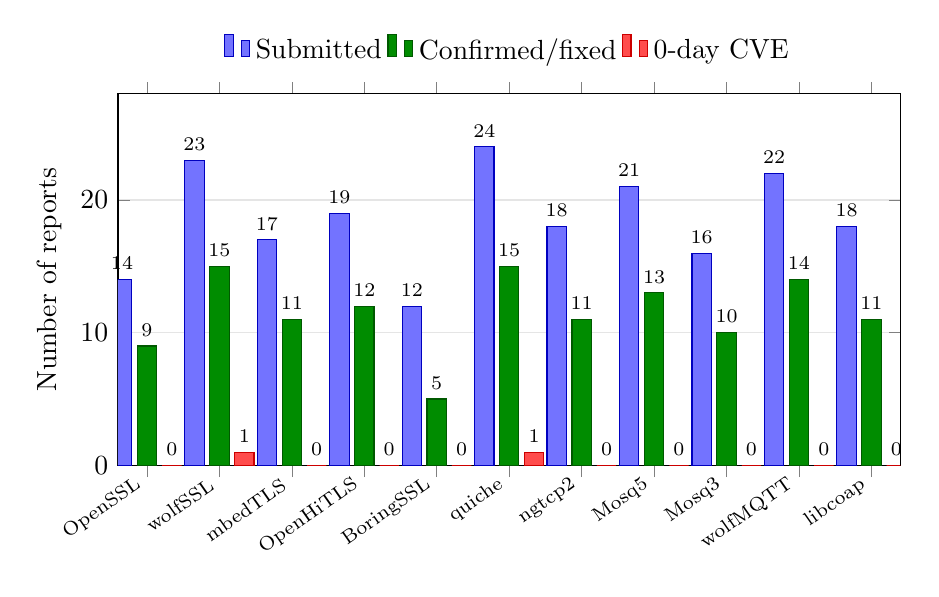
\begin{tikzpicture}
\begin{axis}[
  ybar,
  width=0.95\textwidth,
  height=6.3cm,
  ymin=0,
  ymax=28,
  ylabel={Number of reports},
  symbolic x coords={OpenSSL,wolfSSL,mbedTLS,OpenHiTLS,BoringSSL,quiche,ngtcp2,Mosq5,Mosq3,wolfMQTT,libcoap},
  xtick=data,
  x tick label style={rotate=35, anchor=east, font=\scriptsize},
  legend style={at={(0.5,1.05)}, anchor=south, legend columns=3, draw=none},
  nodes near coords,
  nodes near coords align={vertical},
  nodes near coords style={font=\scriptsize},
  bar width=7pt,
  enlarge x limits=0.04,
  ymajorgrids=true,
  grid style={gray!20},
]
\addplot[fill=blue!55, draw=blue!75!black] coordinates {
  (OpenSSL,14) (wolfSSL,23) (mbedTLS,17) (OpenHiTLS,19) (BoringSSL,12)
  (quiche,24) (ngtcp2,18) (Mosq5,21) (Mosq3,16) (wolfMQTT,22) (libcoap,18)
};
\addplot[fill=green!55!black, draw=green!35!black] coordinates {
  (OpenSSL,9) (wolfSSL,15) (mbedTLS,11) (OpenHiTLS,12) (BoringSSL,5)
  (quiche,15) (ngtcp2,11) (Mosq5,13) (Mosq3,10) (wolfMQTT,14) (libcoap,11)
};
\addplot[fill=red!70, draw=red!80!black] coordinates {
  (OpenSSL,0) (wolfSSL,1) (mbedTLS,0) (OpenHiTLS,0) (BoringSSL,0)
  (quiche,1) (ngtcp2,0) (Mosq5,0) (Mosq3,0) (wolfMQTT,0) (libcoap,0)
};
\legend{Submitted, Confirmed/fixed, 0-day CVE}
\end{axis}
\end{tikzpicture}
\caption{Submitted reports, maintainer-confirmed fixes, and 0-day CVEs by
implementation. The plot separates submitted reports from externally confirmed
fixes so that pending reports are not presented as confirmed bugs.}
\label{fig:bug-bars}
\end{figure*}

\begin{table*}[t]
\centering
\caption{Per-model comparison on conformance inconsistency detection. This
table follows the original GPT/DeepSeek/Claude/Qwen layout while reporting
results per protocol version. Conf. counts maintainer-confirmed fixes, and
Adj.P excludes pending reports from the denominator.}
\label{tab:llm-comparison-implementation-full}
\scriptsize
\setlength{\tabcolsep}{2.7pt}
\begin{tabular}{lr|rrrr|rrrr|rrrr|rrrr|r}
\toprule
\textbf{Protocol}
& \textbf{\#R}
& \multicolumn{4}{c|}{\textbf{GPT-5.4}}
& \multicolumn{4}{c|}{\textbf{DeepSeek}}
& \multicolumn{4}{c|}{\textbf{Claude}}
& \multicolumn{4}{c|}{\textbf{Qwen}}
& \textbf{Avg. Adj.P} \\
\cmidrule(lr){3-6}
\cmidrule(lr){7-10}
\cmidrule(lr){11-14}
\cmidrule(lr){15-18}
& & \textbf{Sub.} & \textbf{Conf.} & \textbf{FP} & \textbf{Adj.P}
& \textbf{Sub.} & \textbf{Conf.} & \textbf{FP} & \textbf{Adj.P}
& \textbf{Sub.} & \textbf{Conf.} & \textbf{FP} & \textbf{Adj.P}
& \textbf{Sub.} & \textbf{Conf.} & \textbf{FP} & \textbf{Adj.P}
& \\
\midrule
TLS 1.3
& 312
& 73 & 47 & 4 & 0.92
& 62 & 37 & 7 & 0.84
& 68 & 42 & 6 & 0.88
& 56 & 31 & 7 & 0.82
& 0.86 \\
QUIC
& 286
& 42 & 26 & 2 & 0.93
& 36 & 21 & 4 & 0.84
& 39 & 24 & 4 & 0.86
& 33 & 18 & 4 & 0.82
& 0.86 \\
MQTT 5.0
& 164
& 21 & 13 & 1 & 0.93
& 18 & 10 & 2 & 0.83
& 19 & 12 & 2 & 0.86
& 17 & 9 & 2 & 0.82
& 0.86 \\
MQTT 3.1.1
& 127
& 38 & 24 & 1 & 0.96
& 32 & 19 & 3 & 0.86
& 34 & 21 & 3 & 0.88
& 28 & 16 & 4 & 0.80
& 0.88 \\
CoAP
& 143
& 18 & 11 & 1 & 0.92
& 16 & 10 & 1 & 0.91
& 17 & 10 & 2 & 0.83
& 15 & 9 & 2 & 0.82
& 0.87 \\
DTLS 1.3
& 198
& 12 & 5 & 0 & 1.00
& 12 & 5 & 1 & 0.83
& 11 & 5 & 2 & 0.71
& 10 & 4 & 2 & 0.67
& 0.80 \\
\bottomrule
\end{tabular}
\end{table*}

For Table~\ref{tab:llm-comparison-implementation-full}, all non-model
components are held fixed: the same extracted rules, retrieval budgets,
validators, adjudication protocol, and test-agent settings are used for every
model. Prompts differ only in model-specific formatting constraints needed to
obtain schema-valid JSON. GPT-5.4 produces the largest number of confirmed
fixes, while smaller or less code-specialized models leave more reports pending
or rejected. Cost differs substantially across providers, so we report cost
only for GPT-5.4, the model used in the main run.

\paragraph{Run-to-run stability.}
Because \tool{} uses LLMs in extraction, filtering, reasoning, and test
planning, we reran the full GPT-5.4 pipeline three times with independent
decoding seeds and empty caches for the LLM stages. Table~\ref{tab:stability}
reports mean and standard deviation over the repeated runs. Deterministic
validators and low-temperature decoding keep variation small, but the
remaining variance is real and is one reason we avoid whole-corpus recall
claims.

\begin{table}[t]
\centering
\caption{Run-to-run stability over three GPT-5.4 runs.}
\label{tab:stability}
\small
\begin{tabular}{lrr}
\toprule
\textbf{Metric} & \textbf{Mean} & \textbf{Std. dev.} \\
\midrule
Submitted reports & 202.7 & 3.1 \\
Confirmed/fixed reports & 124.3 & 2.5 \\
False positives & 9.7 & 1.2 \\
Pending reports & 68.7 & 3.8 \\
Adj.P & 0.93 & 0.01 \\
\bottomrule
\end{tabular}
\end{table}

\subsection{RQ4: Cost Analysis}

Using GPT-5.4 as the cost model, \tool{} spends \$1.122 per submitted report on
average. Since \tool{} submitted 204 reports, the total model cost is
approximately \$228.89. Table~\ref{tab:cost} breaks down the average cost by
stage. Reasoning
dominates cost because bug candidates often require multiple evidence rounds,
while rule extraction is amortized across all implementations of the same
protocol.

\begin{table}[t]
\centering
\caption{Average GPT-5.4 model cost per submitted report.}
\label{tab:cost}
\small
\begin{tabular}{lrr}
\toprule
\textbf{Stage} & \textbf{Cost / Report} & \textbf{Share} \\
\midrule
Rule extraction & \$0.176 & 15.7\% \\
Code-context extraction & \$0.284 & 25.3\% \\
Consistency reasoning & \$0.431 & 38.4\% \\
Verification-test agent & \$0.231 & 20.6\% \\
\midrule
Total & \$1.122 & 100.0\% \\
\bottomrule
\end{tabular}
\end{table}

\subsection{RQ5: Ablation Study}

Table~\ref{tab:ablation} compares system variants using the same adjudication
taxonomy as Table~\ref{tab:verification-results}. Direct Agent submits many
reports but has lower adjudicated precision and covers fewer of the
reference confirmed-fixed reports. Removing code-context extraction or iterative
reasoning reduces the number of reports that maintainers confirm and fix.
Removing the test agent leaves more reports pending because fewer submissions
include executable evidence. The full system covers all 126 reports that are
currently confirmed and fixed and serves as the reference set for the coverage
column; this is \emph{not} a claim of whole-corpus recall, because 69 reports
remain pending and unknown missed bugs are outside the denominator.

\begin{table}[t]
\centering
\caption{Ablation over report status. Cov. is coverage of the 126
confirmed-fixed full-system reports, not global recall.}
\label{tab:ablation}
\small
\setlength{\tabcolsep}{4pt}
\begin{tabular}{lrrrrrl}
\toprule
\textbf{Configuration}
& \textbf{Sub.}
& \textbf{Conf.}
& \textbf{FP}
& \textbf{Pend.}
& \textbf{Adj.P}
& \textbf{Cov.} \\
\midrule
Direct Agent
& 143 & 72  & 24 & 47 & 0.75 & 0.57 \\

w/o Ret \& Test
& 158 & 84  & 18 & 56 & 0.82 & 0.67 \\

w/o Ite Rea
& 176 & 101 & 15 & 60 & 0.87 & 0.80 \\

w/o Test Agent
& 189 & 111 & 14 & 64 & 0.89 & 0.88 \\

Full System
& 204 & 126 & 9  & 69 & 0.93 & Ref. \\
\bottomrule
\end{tabular}
\end{table}

\subsection{Case Studies}

\textbf{Case 1: A TLS implementation accepted an invalid negotiated field.}
\tool{} extracted a MUST-level field constraint from RFC 8446 and mapped it to
a parser state variable in a TLS implementation. The first reasoning round
found only assignment logic, then requested the caller that validates the parsed
value. The resulting report included a minimal transcript and was fixed by the
maintainer.

\textbf{Case 2: A QUIC transport-parameter bug became a 0-day CVE.}
\tool{} identified a missing rejection condition for a boundary value in a QUIC
transport parameter. The test agent generated an input that violated the
standard but was accepted by the implementation. The issue was disclosed and
assigned a CVE after confirmation.

\textbf{Case 3: MQTT version-specific rules prevent false positives.}
MQTT 3.1.1 and MQTT 5.0 have different rule sets. Reusing the wrong rule set
would cause false reports against Mosquitto. \tool{} avoids this by extracting
rules per protocol version and reusing that set only across implementations of
the same version.

\subsection{Failure Analysis}

The unresolved and rejected reports fall into three categories. First, some
pending reports are awaiting maintainer triage even though they include a
reproduction artifact. Second, some pending reports require multi-peer
integration tests that our current validation agent cannot fully automate.
Third, some rejected reports involve intentional compatibility behavior or
SHOULD-level rules that maintainers do not consider bugs. These cases motivate
stronger severity ranking and more protocol-specific test harnesses.

\paragraph{Reviewer-verifiable artifacts.}
Our evaluation is designed to be reviewer-verifiable without de-anonymizing the
authors. Each submitted report is assigned a blinded identifier and linked to:
(i) the normative standard span, (ii) the normalized field rule, (iii) the
implementation evidence category, (iv) the validation status, and (v) the
maintainer/adjudication outcome category. Public identifiers are withheld only
when they would compromise double-blind review. The artifact contains scripts
that reproduce all aggregate tables from the blinded report index. All code,
scripts, and blinded reports are included in an anonymous GitHub artifact
repository submitted with the paper:
\url{https://anonymous.4open.science/r/SpecFSM-Artifact}.
